\section{Uvod}
U ovom radu je na DE1-SoC razvojnom sistemu implementiran jednostavan hardver u FPGA, portovan je Linux operativni sistem i napisan je drajver za pristup registrima i prihvatanje prekida iz FPGA. 

\subsection{Sistemi na čipu sa FPGA}
Sa sve većim mogućnostima namenskih sistema došlo je do popularizacije sistema na čipovima (SoC - System on Chip) koji integrišu mikroprocesore sa više jezgara, memorije na čipu, mnogobrojne periferije i transivere, kao i FPGA (Field Programmable Gate Array).

Ova tehnologija daje dizajneru sistema veliku slobodu i mogućnosti, a zadršava se klasičan postupak projektovanja namenskih sistema. Uz to se ostvaruje veća integracija, manja potrošnja, manja površina štampane ploče (PCB - Printed Circuit Board) i veći protok podataka između procesora i FPGA dela. 

Uobičajena primena ovih sistema je implementacija specifičnih akceleratora koji ubrzavaju izvršavanje algoritama i implementacija specifičnih programabilnih interfejsa ka spoljnom svetu. Nove tehnologije kao što su OpenCL, Vivado HLS, Matlab HDL Coder omogućavaju kompatibilnost dizajna softvera na visokom nivou i implementiranog hardvera na niskom nivou.

SoCFPGA sistemi najčešće sadrže ARM mikroprocesor. Aplikacije na mikroprocesoru bez operativnog sistema (baremetal) nude jednostavno pisanje koda i uštedu na resursima. Za kompleksnije aplikacije koriste se operativni sistemi (OS) i time se olakšava integrisanje mrežnih protokola, rad sa multimedijalnim sadržajima, kriptografskim bibliotekama kao i mnoge druge mogućnosti koje su dostupne kao open-source softver. Kada je potrebno garantovati reakciju u određenom vremenu na neki spoljni događaj veliki operativni sistemi nisu dobro rešenje i koriste operativni sistemi u realnom vremenu (RTOS).

Hardver u FPGA se projektuje upotrebom nekog dva popularna jezika za opis hardvera (Verilog i VHDL - Very High Speed Integrated Circuit Hardwer Description Language) i softverskih alata za specifični uređaj. Dodatno ovi alati olakšavaju dizajn upotrebom IP( Intelectual Property) blokova kao i generisanjem raznih izlaznih fajlova koji opisuju projektovani hardver na standardni način i koriste se prilikom razvoja softvera.

\subsection{Opis DE1-SoC}

U ovom radu korišćen je DE1-SoC razvojni sistem koji se vrlo često upotrebljava u edukativne svrhe. Razvojni sistem je zasnovan na čipu iz familije Cyclone V kompanije Intel (ranije Altera).

U nastavku su navedene samo osobine razvojnog sistema koje se tiču ovog rada, a detaljniji opis se moze pronaći u dokumentu DE1-SoC User Manual []
dodati referencu: \verb+https://www.terasic.com.tw/cgi-bin/page/archive.pl?Language=English&CategoryNo=205&No=836&PartNo=4 +
DE1-SoC User Manual(rev.E Board)
Terasic
\begin{itemize}
\item Sistem na čipu Cyclone V SoC \texttt{5CSEMA5F31}
\item Memorija 1GB (2x256Mx16) DDR3 SDRAM povezana na HPS
\item Slot za Micro SD karticu povezan na HPS
\item UART na USB (USB Mini-B konektor)
\item 5 debaunsiranih tastera (FPGA x4, HPS x1)
\item 11 LE dioda (FPGA x10, HPS x 1)
\item 12V DC napajanje
\end{itemize}

\subsection{Opis Altera Cyclone 5}
Altera Cyclone 5 je SoC FPGA koji se sastoji od dva dela(slika): procesorski deo (HPS -  Hard processor System) i programabilni FGPA deo. HPS se sastoji od MPU (Microprocessor unit) sa ARM Cortex-A9 MPCore sa dva jezgra i sledećih modula: kontroleri memorije, memorije, periferije, sistem interkonekcije, debug moduli, PLL moduli. FPGA deo se sastoji od sledećih delova: FPGA programabilna logika (look-up tabele, RAM memorije, mnozači i rutiranje), kontrolni blok, PLL, kontroler memorije.

Svaki pin kućista je povezan na samo jedan od ova dva dela sistema, tako da HPS deo i FPGA deo ne mogu međusobno razmenjivati pinove.

\subsubsection{Konfigurisanje FPGA i pokretanje HPS}
Pri pokretanju HPS (boot) moze da učita program iz FPGA dela, iz eksterne flash memorije ili preko JTAG. FPGA ima mogućnost da se konfiguriše softverski iz HPS korišćenjem periferije FPGA Manager ili spoljnim programatorom. Kombinacije ovih mogucnosti daju nekoliko scenarija:
\begin{itemize}
\item nezavisno konfigurisanje FPGA i pokretanje HPS
\item konfigurisanje FPGA, zatim pokretanje HPS iz memorije koja se nalazi u FPGA
\item pokretanje HPS, zatim konfigurisanje FPGA iz HPS
\end{itemize}
DE1-SoC razvojni sistem dolazi sa integrisanim programatorom kojem se pristupa preko USB porta. Moguće je podesiti konfigurisanje FPGA spolja ili iz HPS upotrebom prekidača MSEL, dok se HPS uvek pokreće iz flash memorije SD kartice.
(dodati tableu 3-2 iz de1soc user guide)

\subsubsection{HPS-FPGA interfejsi}
HPS-FPGA interfejsi su komunikacioni kanali između HPS i FPGA dela. U nastavku su nabrojani i opisani HPS-FPGA interfejsi:
\begin{itemize}
\item  FPGA-to-HPS bridge - magistrala visokih preformansi konfigurabilne sirine od 32,64 ili 128 bita. Na ovoj magistrali je FPGA master. Ovaj interfejs otkriva FPGA masterima ceo adresni prostor HPS dela.
\item HPS-to-FPGA bridge - magistrala visokih preformansi konfigurabilne sirine od 32,64 ili 128 bita. Na ovoj magistrali je HPS master a u FPGA se nalazi slave.
\item Lightweight HPS-to-FPGA - magistrala sirine 32 bita. HPS je master na ovoj magistrali. Ovaj interfejs manjeg protoka je namenjen za pristup statusnim i kontrolnim registrima periferijama implementiranim u FPGA delu.
\item FPGA manager - HPS periferja koja komunicira sa FPGA delom prilikom konfiguracije ili pokretanja (boot)
\item Prekidi - mogucnost povezivanja prekida iz FPGA na HPS kontroler prekida
\item HPS debug interfejs - omogućava da se debug mogućnosti prošire i na FPGA deo
\end{itemize}

Interfejsi koji su produžetak AXI magistrale na FPGA deo su FPGA-to-HPS bridge, HPS-to-FPGA bridge i Lightweight HPS-to-FPGA. Za povezivanje na ovu magistralu sa strane FPGA koristi se Avalon magistrala, stoga je neophodan AXI-Avalon bridge.

\subsubsection{Proces pokretanja HPS (boot)}
Pokretanje HPS je proces koji se obavlja u više koraka. Nakon izvršavanja svakog koraka se učitava i pokreće sledeći. Ovo je proces je sličan kod svih ARM procesora, a u nastavku je ukratko opisan za konkretnu platformu.

\begin{figure}[h!]
\centering
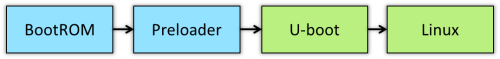
\includegraphics[scale=1.]{img/gsrd-boot.png}
\caption{Tok pokretana sistema}
\label{slika1:gsrd}
\end{figure}

Pri izlazu iz reset stanja procesor počinje izvrsavanje sa reset vektora iz memorije na čipu. Na adresi reset vektora je upisan Boot ROM progtam. Ovo je prvi korak u pokretanju HPS. BootROM izvršava osnovna podešavanja procesora i dohvata Preloader iz NOR flash memorije, NAND flah memorije ili SD/MMC flash memorije. Očitavaju se BSEL pinovi na osnovu kojih se određuje gde je smešten Preloader, zatim se inicijalizuje taj interfejs i učitava i pokreće Preloader. Boot ROM softver proizvođača i ne može se menjati. 

Preloader je prvi korak u pokretanju koji može da se konfiguriše. Preloader koji se koristi u ovom radu je zasnovan na SPL (Secondary Program Loader) framework koji je deo U-Boot projekta, što znači da Preloader i U-Boot dele dosta izvornog koda, kao što je mnoštvo pouzdanih drajvera. Preloader obično izvršava inicijalizaciju SDRAM, dodatna podešavanja sitema, inicijalizaciju flash kontrolera koji sadrži sledeći program (NAND, SD/MMC, QSPI) i zatim učitavanje programa u RAM memoriju i pokretanje.

Softver koji sledi nakon Preloader-a može biti baremetal aplikacija ili bootloader. Preloader i svi prethodni programi se izvršavaju na prvom jezgru procesora dok je drugo u reset stanju. Naredni koraci mogu inicijalizovati drugo jezgro.

Bootloader ima zadatak da podesi promenljive okruženja operativnog sistema, dohvati fajlove za pokretanje operativni sistem (sa flash memorije, putem Etherneta preko TFTP protokola ili USB), konfigurise FPGA pruži konzolu za korisničke operacije. Neki od populatnih open-source bootloadera su U-Boot i Barebox.

\subsection{Alati}
U nastavku će ukratko biti opisani korišćeni alati sa izdvojenim najvažnijim mogućnostima:
\begin{itemize}
\item Quartus Prime 18.0 - alat za razvoj hardvera na FPGA. Deo paketa je Platform Designer (ranije Qsys) koji u dizajn ukljucuje HPS, IP blokove i definiše povezanost ovih delova
\item Preloader Generator (bsp-editor alat iz SoC EDS) - Generise izvorni kod Preloader-a na osnovi izlaznih fajlova koji opisuju hardver
\item Device Tree Generator (sopc2dts alat iz SoC EDS) - Generise Device Tree opis hardvera na osnovi izlaznih fajlova koji opisuju hardver
\item DE1-SoC Builder - Generise prazan Quartus projekat za DE1-SoC razvojni sistem
\item Linaro Toolchain - koristi se za kompajliranje softvera
\end{itemize}

Na slici \ref{slika1:gsrd} je grafički prikazan tok projektovanja jednog SoCFPGA sistema.

\begin{figure}[h!]
\centering
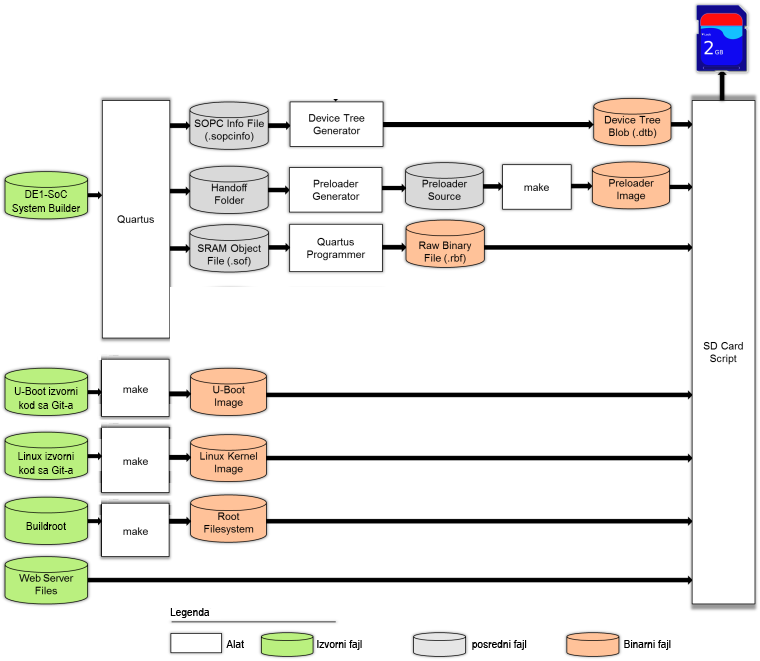
\includegraphics[scale=1.3]{img/gsrd-flow.png}
\caption{Tok projektovanja}
\label{slika1:gsrd}
\end{figure}

U nastavku su objašnjeni fajlovi koji se koriste pri projektovanju:
\begin{itemize}
\item \texttt{.qpf} - projektni fajl za Quartus. Ovaj fajl generiše DE1-SoC Builder
\item \texttt{.qsf} - skripta za podešavanje pinova. Ovaj fajl generiše DE1-SoC Builder
\item \texttt{.sdc} - skripta za podešavanje takta. Ovaj fajl generiše DE1-SoC Builder
\item \texttt{.v} - Verilog HDL izvorni kod
\item \texttt{.vhd} - VHDL izvorni kod
\item \texttt{.sof} -  SDRAM Object File - fajl za programiranje FPGA.  Ovaj fajl generiše Quartus pri kompajliranju dizajna
\item \texttt{.rbf} - Raw Binary File - fajl za programiranje FPGA. Ovaj fajl se dobija konverzijom \texttt{.sof} alatom \texttt{quartus\_cpf}
\item \texttt{.dts} - Device Tree Source - opis hardvera za Linuks kernel
\item \texttt{.dtb} - Device Tree Blob - binarni fajl, kompajlirani opis hardvera za Linuks kernel
\item \texttt{.sopcinfo} - sadrži opis hardvera na osnovu kog se generišu drugi fajlovi. Ovaj fajl generiše Platform Designer
\item \texttt{.c} - izvorni kod u jeziku C
\item \texttt{Makefile} - sadrži set direktiva za \texttt{make buld system}
\end{itemize} 
\pagebreak
\section{Opis projektovanog sistema}

U ovom radu je implementiran jednostavan sistem koji demonstira osnovne mogucnosti u dizajniranju sistema na SoC FPGA. Na slici \ref{slika:q3} je prikazan realizovani sistem (dodati novu sliku?)

\begin{figure}[h!]
\centering
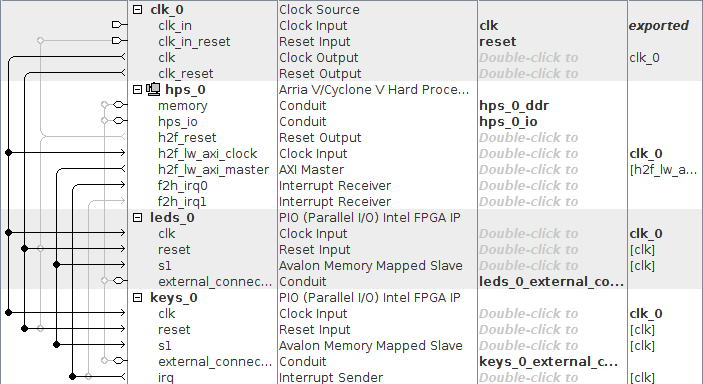
\includegraphics[scale=0.9]{img/quartus3.png}
\caption{Povezivanje \texttt{keys\_0} bloka}
\label{slika:q3}
\end{figure}
\subsection{Memorijski mapiran interfejs ka LE diodama i tasterima u FPGA}
U FPGA delu su postavljena dva PIO (Parallel I/O) Intel FPGA IP bloka. PIO IP blok \texttt{leds\_0} je izlazni i koristi se za kontrolisanje LE dioda. PIO IP blok \texttt{keys\_0} je ulazni i koristi se za očitavanje tastera. PIO IP blok \texttt{keys\_0} takođe šalje prekidni zahtev HPS-u na svaku uzlaznu i silaznu ivicu.

PIO blokovi \texttt{keys\_0} i \texttt{leds\_0} su povezani kao Memory Mapped Slave na Avalon magistralu. Prilikom dizajna se automatski generiše AXI-Avalon bridge i tako su PIO blokovi \texttt{keys\_0} i \texttt{leds\_0} memorijski mapirani u adresni prostor HPS-a.

\subsection{Preloader}
Za pokretanje HPS sistema koristi se Preloader generisan Alterinim alatima na osnovu generisanih fajlova za opis harvera.

\subsection{Bootloader}
Uobicajeni izbor za bootloader je U-Boot. U-Boot  učitava konfiguracioni fajl u \texttt{.rbf} formatu i konfigurise FPGA. Zatim učitava binarni fajl za opis hardverske pratforme (\texttt{.dtb} fajl) i binarni fajl kernela operativnog sistema (\texttt{zImage} fajl). Argumenti za podešavanje sistena se prosleđuju pri prepustanju toka izvršavanja kernelu.

\subsection{Linuks kernel i Root File System}
Izvorni kod za Linuks kernel je preuzet za Alterinog \texttt{git}-a. Root File System je generisan korišćenjem \texttt{buildroot}-a i upisan na SD karticu.

\subsection{Drajver}
Drajver je napisan kao modul kernela koji se uključuje odgovarajućom komandom. Nakon uključivanja drajver iz binarnog opisa harvdera (Device Tree Blob) učitava informacije o harvderu. Drajver pravi fajlove u \texttt{sysfs} fajl sistemu. Čitanje i upis u ove fajlove poziva odgovarajuće funkcije u drajveru koje upravljaju hardverom.

Sistemski fajlovi koje pravi drajver i njihov opis:
\begin{itemize}
\item \texttt{leds} - upisani broj se prikazuje na LE diodama u binarnoj predstavi
\item \texttt{keys} - čitanje vraća binarnu predstavu stanja tastera
\item \texttt{irq\_flag} - pristup registru za flegove prekida (1 na n-tom bitu označava pristigli prekid na n-tom tasteru, upis 1 na n-ti bit čisti n-ti fleg)
\item \texttt{irq\_mask} - čitanje i upis u registar za maksiranje prekida (upis 1 na n-ti bit omogućava prekid na n-tom tasteru)
\end{itemize}

Ceo kod drajvera je dostupan u dodatku.
\subsection*{Testiranje sistema}
Binarni fajlovi za pokretanje sistema i root fajl sistem su napisani na SD karticu. HPS je povezan sa PC računarom preko UART-USB serijske veze. Otvaranjem konzole na PC računaru se pristupa sistemu.\\
U nastavku je dat komplatan spisak koraka za realizovanje sistema.



